\section{Optimizacija s konveksno ovojnico}\label{sec:optimizacija-s-konveksno-ovojnico}

\begin{lstlisting}[label={lst:code4}, language=C++]

for(int stopnja = n - 2; stopnja >= 0; stopnja--) {
    int trenutna_spretnost = spretnost_po[stopnja];

    int64 rezultat = 1e18;

    for(int naslednja_stopnja = stopnja + 1; naslednja_stopnja < n; naslednja_stopnja++) {
        int64 trenutna_vrednost = (int64) trenutna_spretnost * moc_posasti[naslednja_stopnja] + najmanjsi_cas[naslednja_stopnja];

        rezultat = min(rezultat, trenutna_vrednost);
    }

    najmanjsi_cas[stopnja] = rezultat;
}

\end{lstlisting}

Če si bolj natančno pogledamo zgornjo kodo opazimo, da notranja zanka vresnici dobi minimum vseh vrednosti:

\begin{lstlisting}[label={lst:code6}, language=C++]
    trenutna_spretnost * moc_posasti[i] + najmanjsi_cas[i]
\end{lstlisting}

Skozi vse $i$ na intervalu $[stopnja+1, n-1]$.
\\
Če res razmislimo, ugotovimo, da je to enako kot iskanje najmanjšega $y$ na neki množici premic pri nekem $x$.
V tem primeru imamo premice, ki imajo smerni koeficient moc\_posasti[i] in kostanto najmanjsi\_cas[i].
Ko iteriramo v zunanji zanki, se vsako iteracijo doda nova premica: x * moc\_posasti[stopnja + 1] + najmanjsi\_cas[stopnja + 1].
Ostale premice ostanejo.
\\
Zato lahko sprogramiramo podatkovno strukturo, ki nam hrani premice in nam vrne minimum za neki $x$.

\begin{lstlisting}[label={lst:code7}, language=C++]
// standardna knjiznica
#include<iostream>
#include<vector>
// definiramo krajsnjico za 64-bitno stevilo
typedef long long int64;
// da lahko opustimo "std::" predpono
using namespace std;

// Podatkovna struktura, ki hrani premice
struct Premice {
    vector<pair<int64, int64>> premice;

    // dodaj premico y = kx + c
    void dodaj(int64 k, int64 c) {
        premice.push_back({k, c});
    }

    // pridobi nek minimum za nek x
    int64 minimum(int64 x){
        int64 rezultat = 1e18;

        // preprosto izracunaj vse y in najdi najmanjsega
        for(auto [k, c] : premice) {
            rezultat = min(rezultat, k * x + c);
        }

        return rezultat;
    }
};

int n; // stevilo posasti
vector<int> moc_posasti; // moc vsake posasti
vector<int> spretnost_po; // nasa spretnost po uboju vsake posasti
vector<int64> najmanjsi_cas; // tabela namesto funkcije

int main(){
    // ni tako pomembno:
    // preberemo n in x
    int zacetna_spretnost;
    cin>>n>>zacetna_spretnost;
    // nastavimo velikost obeh seznamov na n
    moc_posasti.resize(n);
    spretnost_po.resize(n);
    // preberemo vrednosti in jih vnesemo v oba seznama
    for(int&i:moc_posasti)
        cin>>i;
    for(int&i:spretnost_po)
        cin>>i;

    // rezultat celega programa
    int64 rezultat = 1e18;

    najmanjsi_cas.resize(n);
    najmanjsi_cas[n - 1] = 0;

    // zelo je pomembno, da ko racunamo stopnje, gremo od zadnje do prve,
    // saj pri racunanju uporabimo rezultate poznejsih stopenj

    // tokrat uporabimo podatkovno strukturo
    Premice premice;
    for(int stopnja = n - 2; stopnja >= 0; stopnja--) {
        // koda je precej kratka, saj se vecina zgodi v podatkovni strukturi Premice
        premice.dodaj(moc_posasti[stopnja + 1], najmanjsi_cas[stopnja + 1]);

        najmanjsi_cas[stopnja] = premice.minimum(spretnost_po[stopnja]);
    }

    // prvi uboj je lahko kjerkoli, gremo skozi vse mozne
    for(int prvi_uboj = 0; prvi_uboj < n; prvi_uboj++) {
        int64 trenutna_vrednost = 0;

        // to je cas, ki je potreben, da ubijemo tam bivajoco posast
        trenutna_vrednost += (int64) zacetna_spretnost * moc_posasti[prvi_uboj];

        // poklicemo funkcijo, da nam ugotovi koliko casa bo trajalo, da pridemo do konca
        trenutna_vrednost += najmanjsi_cas[prvi_uboj];

        rezultat = min(rezultat, trenutna_vrednost);
    }

    // rezultat bo na koncu vseboval najkrajsi cas
    // izpisi ga
    cout << rezultat << "\n";

    return 0;
}
\end{lstlisting}

Ta koda ima še vedno časovno zahtevnost $O(n^2)$, vendar pa smo izolirali del kode, ki je odgovoren za iskanje minimuma premic.
Zdaj je pa samo še naloga, da pohitrimo to podatkovno strukturo.

\section{Li Chao drevo}\label{sec:li-chao-drevo}
Opazimo naslednjo stvar: če imamo neko množico premic in nek interval $[l, r]$, in želimo hitro ugotoviti minimum vseh premic za nek x na tem intervalu, lahko to naredimo z Li Chao drevesom.
Najprej definiramo sredino intervala $m = \frac{l + r}{2}$ in najdemo premico, ki ima najmanjši $y$ pri $x = m$.
Rečemo ji središčna premica.
Znano dejstvo je, da se dve različni premici sekata v največ eni točki, zato vemo, da če obstaja tak $x$, da je $y$ neke premice manjši od $y$ središčne premice pri istem $x$, potem na drugi polovici intervala, gotovo ne bo nobenega takega $x$.
Zato lahko rekurzivno razdelimo problem na dva identična problema, vendar z intervaloma $[l, m]$ in $[m, r]$.
Celotna struktura tvori binarno drevo.

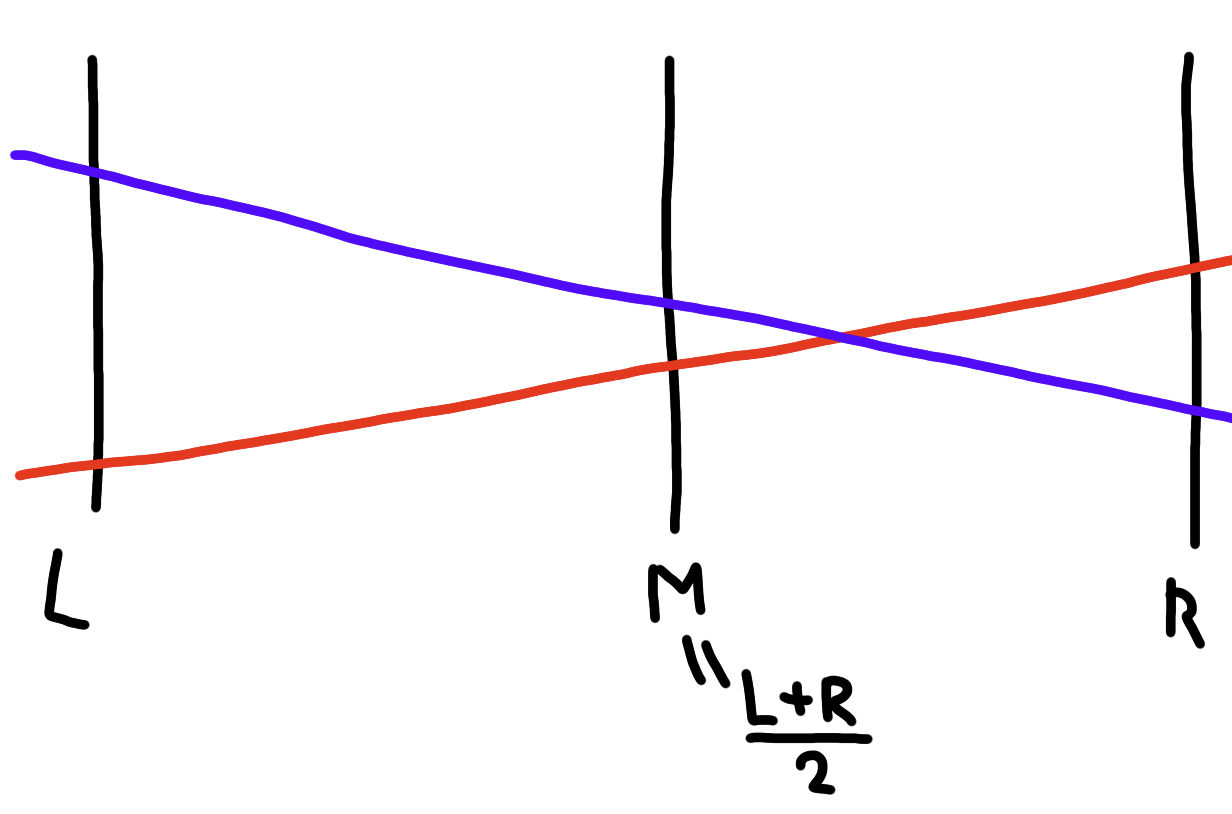
\includegraphics[scale=0.6]{image1}
Slika 1: Slika prikazuje središčno premico in neko drugo premico, ki ima manjši $y$ pri $x = m$.
\\
\\

Tukaj na sliki vidimo, da je središčna premica rdeče obarvana in ima najmanjši $y$ pri $x = m$.
Vijolična premica je neka druga premica, ki po definiciji ne more imeti manjšega $y$ pri $x = m$, zato je lahko manjša od središčne premice samo na enem intervalu.

\begin{lstlisting}[label={lst:code5}, language=C++]
// standardna knjiznica
#include<iostream>
#include<vector>
// definiramo krajsnjico za 64-bitno stevilo
typedef long long int64;
// da lahko opustimo "std::" predpono
using namespace std;

// velikost intervala iz katerega gledamo, v tem primeru vedno gledamo x na intervalu [1, 10^6]
const int VELIKOST = 1<<20;

typedef pair<int64,int64>Premica;

int64 vrednost_premice(int64 x, Premica l) {
    return l.first * x + l.second;
}

// Podatkovna struktura, ki hrani premice
struct Premice{
    vector<Premica> drevo;

    Premice() {
        drevo = vector<Premica>(VELIKOST * 2, {0, 1e18});
    }

    void dodaj(int node, int l, int r, Premica premica) {
        // ce je dolzina intervala 1, ga ne moremo vec deliti
        if(l == r - 1) {
            // glede na to, da gledamo samo se na vrednosti l, lahko vzamemo premico, ki ima manjso vrednost in drugo zavrzemo
            if(vrednost_premice(l, premica) < vrednost_premice(l, drevo[node]))
                drevo[node] = premica;
            return;
        }

        // Poskrbi za robne primere
        if(premica.first > drevo[node].first)
            swap(premica, drevo[node]);

        int m = (l + r) / 2;
        // v drugem primeru pogledamo, ce je trenutna premica nasa premica primerna za srediscno premico
        if(vrednost_premice(m, premica) < vrednost_premice(m, drevo[node])) {
            // zamenjamo, da je zdaj ta srediscna in prejsnjo srediscno premico potisnemo dol
            swap(premica, drevo[node]);
            dodaj(2 * node, l, m, premica);
        } else
            // v nasprotnem primeru potisnemo na drugo stran
            dodaj(2 * node + 1, m, r, premica);
    }

    void dodaj(Premica l) {
        dodaj(1, 0, VELIKOST, l);
    }

    int64 minimum(int node, int l, int r, int64 x) {\
        // ce je dolzina intervala 1, ga ne moremo vec deliti
        if(l == r - 1)
            return vrednost_premice(x, drevo[node]);


        int m = (l + r) / 2;
        // najprej evaluiramo trenutno premico
        int64 val = vrednost_premice(x, drevo[node]);

        // potem pa gremo na primerno stran
        if(x < m)
            val = min(val, minimum(2 * node, l, m, x));
        else
            val = min(val, minimum(2 * node + 1, m, r, x));
        return val;
    }

    int64 minimum(int64 x) {
        return minimum(1, 0, VELIKOST, x);
    }
};

int n; // stevilo posasti
vector<int> moc_posasti; // moc vsake posasti
vector<int> spretnost_po; // nasa spretnost po uboju vsake posasti
vector<int64> najmanjsi_cas; // tabela namesto funkcije

int main(){
    // ni tako pomembno:
    // preberemo n in x
    int zacetna_spretnost;
    cin>>n>>zacetna_spretnost;
    // nastavimo velikost obeh seznamov na n
    moc_posasti.resize(n);
    spretnost_po.resize(n);
    // preberemo vrednosti in jih vnesemo v oba seznama
    for(int&i:moc_posasti)
        cin>>i;
    for(int&i:spretnost_po)
        cin>>i;

    // rezultat celega programa
    int64 rezultat = 1e18;

    najmanjsi_cas.resize(n);
    najmanjsi_cas[n - 1] = 0;

    // zelo je pomembno, da ko racunamo stopnje, gremo od zadnje do prve,
    // saj pri racunanju uporabimo rezultate poznejsih stopenj

    // tokrat uporabimo podatkovno strukturo
    Premice premice;
    for(int stopnja = n - 2; stopnja >= 0; stopnja--) {
        // koda je precej kratka, saj se vecina zgodi v podatkovni strukturi Premice
        premice.dodaj({moc_posasti[stopnja + 1], najmanjsi_cas[stopnja + 1]});

        najmanjsi_cas[stopnja] = premice.minimum(spretnost_po[stopnja]);
    }

    // prvi uboj je lahko kjerkoli, gremo skozi vse mozne
    for(int prvi_uboj = 0; prvi_uboj < n; prvi_uboj++) {
        int64 trenutna_vrednost = 0;

        // to je cas, ki je potreben, da ubijemo tam bivajoco posast
        trenutna_vrednost += (int64) zacetna_spretnost * moc_posasti[prvi_uboj];

        // poklicemo funkcijo, da nam ugotovi koliko casa bo trajalo, da pridemo do konca
        trenutna_vrednost += najmanjsi_cas[prvi_uboj];

        rezultat = min(rezultat, trenutna_vrednost);
    }

    // rezultat bo na koncu vseboval najkrajsi cas
    // izpisi ga
    cout << rezultat << "\n";

    return 0;
}
\end{lstlisting}